\documentclass[11pt,a4paper]{article}
\usepackage[margin=0.50in]{geometry}
\usepackage[T1]{fontenc}
\usepackage[utf8]{inputenc}
\usepackage{lmodern}
\usepackage{amsmath}
\usepackage{booktabs}
\usepackage{array}
\usepackage{tabularx}
\usepackage{enumitem}
\usepackage{hyperref}
\usepackage{parskip}
\usepackage{tikz}
\usetikzlibrary{arrows.meta,positioning}
\linespread{0.93}
\setlist[itemize]{leftmargin=1.2em, itemsep=0pt, topsep=1pt}
\setlength{\parskip}{2pt}
\setlength{\parindent}{0pt}
\pagestyle{plain}

\title{\vspace{-8pt}\textbf{ArXiv Research Field Activity Analysis Using Hadoop MapReduce}\vspace{-4pt}}
\author{%
  \normalsize University of Ruhuna \textemdash{} Faculty of Engineering\\[1pt]
  \normalsize EE7222/EC7204 Cloud Computing \quad|\quad Group 46\\[3pt]
  \small Ashfaq MRM\,(EG/2021/4417) \quad
         Dissanayake WMNP\,(EG/2021/4499) \quad
         Munsif MFA\,(EG/2021/4684)%
}
\date{\today}

\begin{document}
\maketitle
\vspace{-12pt}

\section*{1. Objective}
This project analyzes the ArXiv metadata snapshot using Hadoop MapReduce in a pseudo-distributed single-node environment. For each research category the job computes total paper count, average version count, average abstract length, and average author count. The dataset is naturally suited for MapReduce because each paper can belong to multiple categories, forming a many-to-many aggregation problem across 2.2 million records.

\section*{2. Dataset and Environment}
The input is the Cornell University ArXiv metadata snapshot (Kaggle), stored in HDFS as JSON Lines — one complete JSON object per line. Each record contains: \texttt{categories}, \texttt{versions}, \texttt{abstract}, and \texttt{authors\_parsed}. The implementation ran in WSL2 (Ubuntu~22.04) using Java~11, Hadoop~3.3.6, HDFS, YARN, and Maven with a fat JAR built via the assembly plugin.

\section*{3. MapReduce Design}

\textbf{Pipeline Overview:}
\vspace{3pt}
\begin{center}
  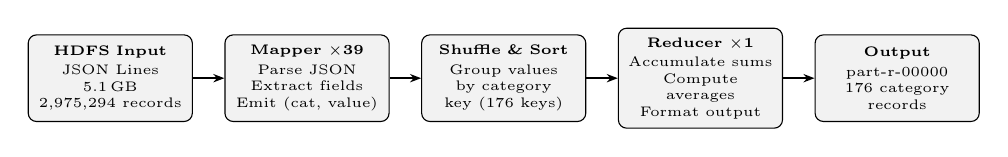
\begin{tikzpicture}[
    node distance=0.40cm,
    box/.style={draw, rounded corners=3pt, fill=gray!10, font=\tiny,
        text width=1.85cm, align=center, minimum height=1.10cm},
    arr/.style={-{Stealth[length=4pt]}, thick}
    ]
    \node[box] (input)  {\textbf{HDFS Input}\\[1pt]JSON Lines\\5.1\,GB\\2,975,294 records};
    \node[box, right=of input]   (map)     {\textbf{Mapper $\times$39}\\[1pt]Parse JSON\\Extract fields\\Emit (cat, value)};
    \node[box, right=of map]     (shuffle) {\textbf{Shuffle \& Sort}\\[1pt]Group values\\by category\\key (176 keys)};
    \node[box, right=of shuffle] (reduce)  {\textbf{Reducer $\times$1}\\[1pt]Accumulate sums\\Compute averages\\Format output};
    \node[box, right=of reduce]  (output)  {\textbf{Output}\\[1pt]part-r-00000\\176 category\\records};
    \draw[arr] (input)  -- (map);
    \draw[arr] (map)    -- (shuffle);
    \draw[arr] (shuffle)-- (reduce);
    \draw[arr] (reduce) -- (output);
  \end{tikzpicture}
\end{center}
\vspace{1pt}

\textbf{Mapper} parses one JSON object per line, extracts category codes, version count, abstract word count, and author count. For every category a paper belongs to, it emits:
\begin{center}
  \texttt{(category,\ "1\,|\,versionCount\,|\,abstractWords\,|\,authorCount")}
\end{center}
This allows one paper to contribute to multiple fields (e.g.\ \texttt{cs.LG} and \texttt{cs.AI}) simultaneously.

\textbf{Reducer} aggregates raw counts per category and computes:
\[
  \text{avgVersions}=\frac{\sum v_i}{N},\quad
  \text{avgAbstractWords}=\frac{\sum w_i}{N},\quad
  \text{avgAuthors}=\frac{\sum a_i}{N}
\]
where $N$ is the total paper count for that category. Averages are deferred entirely to the reducer, making the design combiner-safe with no intermediate precision loss.

\section*{4. Execution Summary}
The final YARN run completed in approximately 2 minutes and 11 seconds. Key job counters:
\begin{itemize}
  \item Map input records: 2,975,294 \quad|\quad Map tasks: 39 \quad|\quad Reduce tasks: 1
  \item HDFS bytes read: 5,142,915,425 \quad|\quad Throughput: $\approx$22,700 records/sec
  \item Total categories in output: 176 \quad|\quad Malformed/skipped records: 0
\end{itemize}

\begin{table}[ht]
  \centering
  \caption{Representative Output --- Selected to Highlight Metric Extremes Across Fields}
  \label{tab:sample}
  \small
  \begin{tabularx}{\linewidth}{@{}lrrrr@{}}
    \toprule
    Category             & Total Papers & Avg Versions  & Avg Words    & Avg Authors   \\
    \midrule
    \texttt{cs.LG}       & 256,056      & 1.70          & 172          & 4.4           \\
    \texttt{cs.CV}       & 183,697      & 1.60          & 177          & 5.1           \\
    \texttt{hep-ph}      & 194,235      & 1.71          & 124          & 3.7           \\
    \texttt{hep-th}      & 180,439      & 1.86          & 121          & 2.4           \\
    \texttt{hep-ex}      & 59,386       & 1.70          & 130          & \textbf{33.5} \\
    \texttt{astro-ph.GA} & 75,811       & 1.42          & \textbf{217} & 9.1           \\
    \texttt{math.AG}     & 58,593       & 1.93          & \textbf{92}  & 1.8           \\
    \texttt{econ.EM}     & 5,149        & \textbf{2.12} & 152          & 2.5           \\
    \bottomrule
  \end{tabularx}
\end{table}

\section*{5. Interpretation of Results}

\textbf{Patterns \& Insights.}~The output reveals four behavioral axes across 176 categories. (i)~\textit{Scale:} \texttt{cs.LG} (256K papers) is the largest category, driven by the post-2015 deep learning boom, followed by \texttt{hep-ph} (194K) and \texttt{cs.CV} (184K). (ii)~\textit{Collaboration:} The author-count axis shows the widest spread --- experimental physics (\texttt{hep-ex}: 33.5 authors, \texttt{nucl-ex}: 16.9, \texttt{astro-ph.IM}: 14.0) reflects large-detector consortia (LHC, ALMA), while pure mathematics (\texttt{math.AG}, \texttt{math.DG}) averages 1.8--1.9, typical of solo theoretical work. (iii)~\textit{Abstract length:} Astrophysics sub-categories write the longest abstracts (\texttt{astro-ph.GA}: 217 words, \texttt{astro-ph.EP}: 209) because observational papers describe instruments and datasets, whereas pure math abstracts (\texttt{math.AG}: 92, \texttt{math.CV}: 89) rely on symbolic notation over prose. (iv)~\textit{Revision behavior:} Economics has the highest revision rates (\texttt{econ.EM}: 2.12, \texttt{econ.TH}: 2.03), reflecting iterative peer-review cycles, while legacy deprecated categories (\texttt{acc-phys}: 49 papers, avg 1.10; \texttt{plasm-ph}: 38 papers, avg 1.13) show near-zero revision activity.

\textbf{Performance.}~On a single WSL2 node the job sustained $\approx$22,700 records/sec and read 5.1\,GB in 131 seconds. The 39 map splits arose automatically from Hadoop's default 128\,MB block size. The single reducer handled 176 unique keys and completed in under 10 seconds of reduce time. Error counters recorded zero malformed JSON lines and zero missing-category records, confirming full dataset coverage.

\section*{6. Future Extensions}
\begin{itemize}
  \item \textbf{Temporal trends:} Partition mapper output by submission year (from \texttt{versions[0].created}) to compute year-over-year growth rates per category.
  \item \textbf{Distributed scale-out:} Deploy on a multi-node YARN cluster (AWS EMR or GCP Dataproc) with multiple reducers partitioned by category prefix to remove the single-reducer bottleneck.
  \item \textbf{NLP enrichment:} Chain a second MapReduce job on the \texttt{abstract} field to compute per-category TF-IDF keyword scores or latent semantic topics, enabling automatic field labeling.
\end{itemize}

\section*{7. MapReduce Logic Pseudocode}
 {\footnotesize
  \begin{flushleft}
    \textbf{--- MAPPER ---}\quad
    \texttt{map(key, jsonLine):}\\
    \hspace*{1em}\texttt{if line empty or JSON invalid $\Rightarrow$ increment errorCounter; return}\\
    \hspace*{1em}\texttt{cats $\leftarrow$ json["categories"].split(" ");\quad if empty $\Rightarrow$ skip}\\
    \hspace*{1em}\texttt{v $\leftarrow$ versions.length;\quad w $\leftarrow$ wordCount(abstract);\quad a $\leftarrow$ authors\_parsed.length}\\
    \hspace*{1em}\texttt{for each cat in cats: emit(cat, "1|v|w|a")}\\[2pt]
    \textbf{--- REDUCER ---}\quad
    \texttt{reduce(category, values):}\\
    \hspace*{1em}\texttt{N, sumV, sumW, sumA $\leftarrow$ 0}\\
    \hspace*{1em}\texttt{for each val in values: parse (c,v,w,a); N+=c;\; sumV+=v;\; sumW+=w;\; sumA+=a}\\
    \hspace*{1em}\texttt{if N=0: return;\quad emit(category, "total=N | avg\_ver=sumV/N | avg\_words=sumW/N | avg\_authors=sumA/N")}
  \end{flushleft}
 }

\end{document}
